\chapter{Estado de la Cuestión}
\label{cap:estadoDeLaCuestion}




\section{Cuestiones básicas de inmunología}

Antes de comenzar sería conveniente introducir una serie de definiciones y explicaciones básicas referentes al sistema inmune y a los procesos que este lleva a cabo. De esta manera, los conceptos y modelos que se expondrán más adelante serán entendidos en su contexto y sin ningún impedimento terminológico. 

Haremos un recorrido desde lo más básico, comenzando por el sistema inmmune innato, e iremos aumentando nuestro nivel de conocimiento en este ámbito poco a poco. 

\subsection{El sistema inmune innato}
Como ya hemos comentado en la Sección \ref{cap:introduccion} de Introducción, el sistema inmune funciona como un equipo. Está compuesto por numerosas células, proteínas y otros agentes de distinto tipo que trabajan de forma coordinada para dar una respuesta eficaz y proporcional al ataque recibido. Pero comencemos por lo más simple: las barreras físicas. La piel y la mucosa de nuestro sistema respiratorio, digestivo y reproductivo intentan que virus, bacterias, hongos o parásitos entren en nuestro organismo. Pero, ¿qué pasa si estos logran atravesar esta barrera?

Aquí entra lo que se denomina \textit{sistema inmune innato}, este recibe este nombre porque parece la defensa ``natural'' que todo animal parece tener. De hecho, muchos mecanismos de este sistema inmune innato llevan con nosotros más de 500 millones de años. 
Entre los componentes más famosos de este sistema encontramos los \textit{macrófagos}. Su nombre compuesto por ``\textit{macro}'', que significa grande y ``\textit{fago}'', que significa comer, lo dice todo. En efecto, los macrófagos son células que se comen invasores mediante un proceso llamado \textit{fagocitosis}, que ilustra la Figura \ref{fig:macrofago}. El mecanismo es muy similar al utilizado por una ameba. Una vez que el \textit{macrófago} tiene en un interior a la bacteria, la degrada en una vesícula llamada \textit{lisosoma}. Esta contiene sustancias que podrían degradar hasta el propio \textit{macrófago} si salieran de esta vesícula. 


\begin{figure}[t]
	\centering
	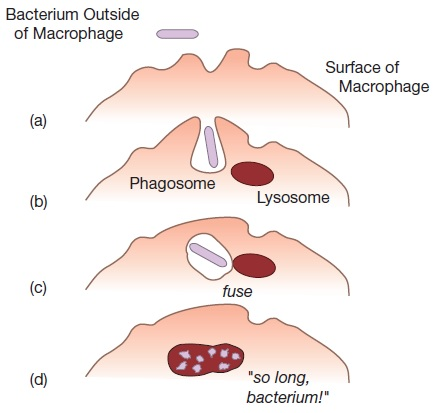
\includegraphics[width=0.5\textwidth]{1_macrofago}
	\caption{Fagocitación de un macrófago a una bacteria.}
	\label{fig:macrofago}
\end{figure}


Durante la batalla con las bacterias, los \textit{macrófagos} producen y secretan unas proteínas llamadas \textit{citoquinas}.
Estas son hormonas que facilitan la comunicación entre células del SI y cobrarán un papel muy relevante en los capítulos que siguen.
Podríamos decir que los \textit{macrófagos} hacen el papel de centinelas, que cuando ven al enemigo mandan señales (\textit{citoquinas}) para reclutar a más defensores. A continuación, veremos otros tipos de células, en este caso referentes al \textit{sistema inmune adaptativo}.

\subsection{El sistema inmune adaptativo}

El nombre es bastante descriptivo y, valga la redundancia, gracias a este SI somos capaces de adaptar nuestras defensas contra nuevos invasores. Pero no fue hasta los años 70 cuando tuvimos constancia de esta habilidad adaptativa. Por aquel entonces Edward Jenner comenzó a vacunar a la población inglesa contra el virus de la viruela, en esa época este virus fue la causa de numerosas muertes y desfiguraciones. Lo que Jenner observó es que los ganaderos que se dedicaban a ordeñar vacas contraían el virus de la viruela bovina (\textit{cowpox, en inglés}) y que, aquellos  que habían contraído el virus bovino, raramente contraían la viruela. Así que Jenner decidió llevar a cabo un experimento: guardó pus de uno de los ganaderos con viruela bovina y lo usó para inocular a un niño sano, James Phipps. Después Phipps fue reinoculado con pus proveniente de una persona con viruela, pero no contrajo la enfermedad. De esta manera, quizá poco ortodoxa, Jenner demostró que el sistema inmune humano podía proporcionar armas para protegernos de un intruso que no había visto antes. Lo que debemos remarcar es que la vacuna contra la viruela solo protegía contra esta enfermedad o algunas causadas por virus similares, como en el caso de la viruela bovina. Es decir, el SI adaptativo se adapta para defendernos de invasores específicos. 

Veamos ahora qué forma tienen estos invasores: seguro que el término \textit{anticuerpo} no resulta desconocido, pero ¿a qué nos referimos con él? Los \textit{anticuerpos} no son más que proteínas especiales que circulan por la sangre, y el agente que hace que se produzcan se denomina \textit{antígeno} (en el ejemplo anterior, el \textit{antígeno}, sería el virus de la viruela). Gracias a su estructura, los \textit{anticuerpos} son capaces de encajar en un determinado \textit{antígeno}, como vemos en la Figura \ref{fig:macrofago_anticuerpo}. Los anticuerpos son producidos por unas células inmunes conocidas, las células B. Este tipo de células empiezan con el mismo ADN, pero cuando empiezan a madurar el ADN que forma los anticuerpos puede cambiar. Dando lugar así a gran diversidad de ellos y permitiendo la adaptabilidad de nuestro SI.

La misión principal de los \textit{anticuerpos} es identificar a los ``indeseables'', dejando que el trabajo sucio lo hagan otros. Es decir, gracias a la presencia de \textit{anticuerpos}, otras células, como los ya conocidos \textit{macrófagos} son capaces de identificar a los atacantes. Pero... ¿qué ocurre cuando un virus ya ha entrado en una célula de nuestro cuerpo? Los \textit{anticuerpos} no pueden alcanzarlo y el virus puede dedicarse a replicarse cuanto quiera. En este momento, es el turno de las células protagonistas de este trabajo, las células T. 

\subsubsection{Las células T}
Como las células B, las células T se producen en la médula y maduran en el timo, de ahí la T de su nombre. Su superficie consta de unas moléculas que permiten la interacción con los \textit{anticuerpos} llamados receptores (TCR, \textit{T Cell Receptors}). Hay distintos tipos de células T atendiendo al papel que desempeñan: las células T-Helper secretan \textit{citoquinas} con el objetivo de avisar y activar a otras células inmunitarias, por su parte las células T-killer son un arma muy potente, pues pueden destruir células infectadas. La manera que tienen de acabar con los virus es haciendo que las células infectadas con ellos se suiciden, de esta forma tanto el virus como la célula infectada mueren.

Cuando las células T salen del timo se encuentran desactivadas, en un estado naïve y se dedican a circular por los órganos linfoides secundarios, cuyo máximo representante es el nodo linfático. Allí se encuentran con células provenientes del foco de una infección, que han fagocitado a algún agente infeccioso. Estas presentan en su membrana ciertos \textit{antígenos}, que son reconocidos por las células T gracias a su TCR. Si este \textit{antígeno} se reconoce como extraño, la célula T se activa, convirtiéndose así en una célula efectora, capaz de secretar \textit{citoquinas} y de ir a la zona afectada a combatir al agente extraño.



\begin{figure}[t]
	\centering
	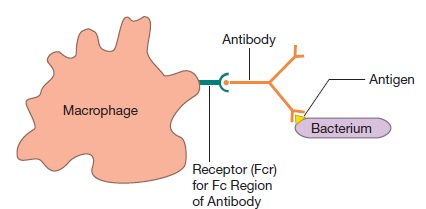
\includegraphics[width=0.5\textwidth]{2_macrofago_anticuerpo}
	\caption{Macrófago reconociendo una bacteria gracias a la acción anticuerpo-antígeno.}
	\label{fig:macrofago_anticuerpo}
\end{figure}


 